%
% Main document
% ===========================================================================
% This is part of the document "Project documentation template".
% Authors: brd3, kaa1
%

%---------------------------------------------------------------------------
\documentclass[
	a4paper,					% paper format
	10pt,							% fontsize
%	twoside,					% double-sided
	openright,				% begin new chapter on right side
	notitlepage,			% use no standard title page
	parskip=half,			% set paragraph skip to half of a line
]{scrreprt}					% KOMA-script report
%---------------------------------------------------------------------------

\raggedbottom
\KOMAoptions{cleardoublepage=plain}			% Add header and footer on blank pages


% Load Standard Packages:
%---------------------------------------------------------------------------
\usepackage[standard-baselineskips]{cmbright}

\usepackage[ngerman]{babel}										% german hyphenation
\usepackage[utf8]{inputenc}  							% Unix/Linux - load extended character set (ISO 8859-1)
%\usepackage[ansinew]{inputenc}  							% Windows - load extended character set (ISO 8859-1)
\usepackage[T1]{fontenc}											% hyphenation of words with ä,ö and ü
\usepackage{textcomp}													% additional symbols
\usepackage{ae}																% better resolution of Type1-Fonts 
\usepackage{fancyhdr}													% simple manipulation of header and footer 
\usepackage{etoolbox}													% color manipulation of header and footer
\usepackage{graphicx}                      		% integration of images
\usepackage{float}														% floating objects
\usepackage{caption}													% for captions of figures and tables
\usepackage{booktabs}													% package for nicer tables
\usepackage{tocvsec2}													% provides means of controlling the sectional numbering
%---------------------------------------------------------------------------

% Load Math Packages
%---------------------------------------------------------------------------
\usepackage{amsmath}                    	   	% various features to facilitate writing math formulas
\usepackage{amsthm}                       	 	% enhanced version of latex's newtheorem
\usepackage{amsfonts}                      		% set of miscellaneous TeX fonts that augment the standard CM
\usepackage{amssymb}													% mathematical special characters
\usepackage{exscale}													% mathematical size corresponds to textsize
%---------------------------------------------------------------------------

% Package to facilitate placement of boxes at absolute positions
%---------------------------------------------------------------------------
\usepackage[absolute]{textpos}
\setlength{\TPHorizModule}{1mm}
\setlength{\TPVertModule}{1mm}
%---------------------------------------------------------------------------					
			
% Definition of Colors
%---------------------------------------------------------------------------
\RequirePackage{color}                          % Color (not xcolor!)
\definecolor{linkblue}{rgb}{0,0,0.8}            % Standard
\definecolor{darkblue}{rgb}{0,0.08,0.45}        % Dark blue
\definecolor{bfhgrey}{rgb}{0.41,0.49,0.57}      % BFH grey
%\definecolor{linkcolor}{rgb}{0,0,0.8}     			% Blue for the web- and cd-version!
\definecolor{linkcolor}{rgb}{0,0,0}        			% Black for the print-version!
%---------------------------------------------------------------------------

% Hyperref Package (Create links in a pdf)
%---------------------------------------------------------------------------
\usepackage[
	pdftex,ngerman,bookmarks,plainpages=false,pdfpagelabels,
	backref = {false},										% No index backreference
	colorlinks = {true},                  % Color links in a PDF
	hypertexnames = {true},               % no failures "same page(i)"
	bookmarksopen = {true},               % opens the bar on the left side
	bookmarksopenlevel = {0},             % depth of opened bookmarks
	pdftitle = {Template für Bachelor Thesis},	   	% PDF-property
	pdfauthor = {brd3},        					  % PDF-property
	pdfsubject = {LaTeX Template},        % PDF-property
	linkcolor = {linkcolor},              % Color of Links
	citecolor = {linkcolor},              % Color of Cite-Links
	urlcolor = {linkcolor},               % Color of URLs
]{hyperref}
%---------------------------------------------------------------------------
% Set up page dimension
%---------------------------------------------------------------------------
\usepackage{geometry}
\geometry{
	a4paper,
	left=28mm,
	right=15mm,
	top=30mm,
	headheight=20mm,
	headsep=10mm,
	textheight=242mm,
	footskip=15mm
}
%---------------------------------------------------------------------------

% Makeindex Package
%---------------------------------------------------------------------------
\usepackage{makeidx}                         		% To produce index
\makeindex                                    	% Index-Initialisation
%---------------------------------------------------------------------------

% Glossary Package
%---------------------------------------------------------------------------
% the glossaries package uses makeindex
% if you use TeXnicCenter do the following steps:
%  - Goto "Ausgabeprofile definieren" (ctrl + F7)
%  - Select the profile "LaTeX => PDF"
%  - Add in register "Nachbearbeitung" a new "Postprozessoren" point named Glossar
%  - Select makeindex.exe in the field "Anwendung" ( ..\MiKTeX x.x\miktex\bin\makeindex.exe )
%  - Add this [ -s "%tm.ist" -t "%tm.glg" -o "%tm.gls" "%tm.glo" ] in the field "Argumente"
%
% for futher informations go to http://ewus.de/tipp-1029.html
%---------------------------------------------------------------------------
\usepackage[nonumberlist]{glossaries}
\makeglossaries

\newglossaryentry{BibTeX}{name={BibTeX},description={Programm zur Erstellung von Literaturangaben und -verzeichnissen in \TeX- oder \LaTeX-Dokumenten}}
\newglossaryentry{StwVrz}{name={Stichwortverzeichnis},description={Verzeichnis mit Stichworten aus dem Text}}



%---------------------------------------------------------------------------

% Intro:
%---------------------------------------------------------------------------
\begin{document}                              	% Start Document
\settocdepth{section}														% Set depth of toc
\pagenumbering{roman}														
%---------------------------------------------------------------------------

\providecommand{\titel}{Telemetrie für Projekt Bern Formula Students}		%  Hier den Titel des Berichts/Thesis eingeben					% Titel der Arbeit aus Datei titel.tex lesen
\providecommand{\versionnumber}{0.4}			%  Hier die aktuelle Versionsnummer eingeben
\providecommand{\versiondate}{14.06.2015}		%  Hier das Datum der aktuellen Version eingeben
				% Versionsnummer und -datum aus Datei version.tex lesen

% Set up header and footer
%---------------------------------------------------------------------------
\makeatletter
\patchcmd{\@fancyhead}{\rlap}{\color{bfhgrey}\rlap}{}{}		% new color of header
\patchcmd{\@fancyfoot}{\rlap}{\color{bfhgrey}\rlap}{}{}		% new color of footer
\makeatother

\fancyhf{}																		% clean all fields
\fancypagestyle{plain}{												% new definition of plain style	
	\fancyfoot[OR,EL]{\footnotesize \thepage} 	% footer right part --> page number
	\fancyfoot[OL,ER]{\footnotesize \titel, Version \versionnumber, \versiondate}	% footer even page left part 
}

\renewcommand{\chaptermark}[1]{\markboth{\thechapter.  #1}{}}
\renewcommand{\headrulewidth}{0pt}				% no header stripline
\renewcommand{\footrulewidth}{0pt} 				% no bottom stripline

\pagestyle{plain}
%---------------------------------------------------------------------------


% Title Page and Abstract
%---------------------------------------------------------------------------
%
% Project documentation template
% ===========================================================================
% This is part of the document "Project documentation template".
% Authors: brd3, kaa1
%

\begin{titlepage}


% BFH-Logo absolute placed at (28,12) on A4 
% Actually not a realy satisfactory solution but working.
%---------------------------------------------------------------------------
\setlength{\unitlength}{1mm}
\begin{textblock}{20}[0,0](28,12)
	
\includegraphics[scale=1.0]{bilder/BFH_Logo_B.png}
\end{textblock}
\color{black}

% Institution / Titel / Untertitel / Autoren / Experten:
%---------------------------------------------------------------------------
\begin{flushleft}

\vspace*{21mm}

\fontsize{26pt}{40pt}\selectfont 
\titel 				\\							% Titel aus der Datei vorspann/titel.tex lesen
\vspace{2mm}

\fontsize{16pt}{24pt}\selectfont\vspace{0.3em}
Hier steht ein Untertitel 			\\							% Untertitel eingeben
\vspace{5mm}

\fontsize{10pt}{12pt}\selectfont
\textbf{Projekt 2} \\									% eingeben
\vspace{7mm}

% Abstract (eingeben):
%---------------------------------------------------------------------------
\begin{textblock}{150}(28,100)
\fontsize{10pt}{12pt}\selectfont
[Kurztext (Abstract) einfügen, falls gewünscht] \\ 
Dieses Dokument dient als Vorlage für die Erstellung von Berichten nach den Richtlinien der BFH. Die Vorlage ist in \LaTeX{} erstellt und unterstützt das automatische Erstellen von diversen Verzeichnissen, Literaturangaben, Indexierung und Glossaren. Dieser kleine Text ist eine Zusammenfassung über das vorliegenden Dokument mit einer Länge von 4 bis max. 8 Zeilen. \\
Das Titelbild kann in den Zeilen 157/158 der Datei template.tex ein- oder ausgeschaltet werden.
\end{textblock}

\begin{textblock}{150}(28,225)
\fontsize{10pt}{17pt}\selectfont
\begin{tabbing}
xxxxxxxxxxxxxxx\=xxxxxxxxxxxxxxxxxxxxxxxxxxxxxxxxxxxxxxxxxxxxxxx \kill
Studiengang:	\> Informatik	\\			% Namen eingeben
Autoren:		\> Pascal Bohni, Roger Jaggi		\\					% Namen eingeben
Betreuer:	\> Dr.~Andreas Danuser		\\					% Namen eingeben
%Auftraggeber:	\> [Wwwww AG]						\\					% Namen eingeben
%Experten:		\> [Dr.~Zzzz Zzzz]				\\					% Namen eingeben
Datum:			\> \versiondate					\\		% aus Datei vorspann/version.tex lesen
\end{tabbing}

\end{textblock}
\end{flushleft}

\begin{textblock}{150}(28,280)
\noindent 
\color{bfhgrey}\fontsize{9pt}{10pt}\selectfont
Berner Fachhochschule | Haute école spécialisée bernoise | Bern University of Applied Sciences
\color{black}\selectfont
\end{textblock}


\end{titlepage}

%
% ===========================================================================
% EOF
%
		% activate for Titelseite ohne Bild
%%
% Project documentation template
% ===========================================================================
% This is part of the document "Project documentation template".
% Authors: brd3, kaa1
%

\begin{titlepage}


% BFH-Logo absolute placed at (28,12) on A4 and picture (16:9 or 15cm x 8.5cm)
% Actually not a realy satisfactory solution but working.
%---------------------------------------------------------------------------
\setlength{\unitlength}{1mm}
\begin{textblock}{20}[0,0](28,12)
	
\includegraphics[scale=1.0]{bilder/BFH_Logo_B.png}
\end{textblock}

\begin{textblock}{154}(28,48)
	\begin{picture}(150,2)
		\put(0,0){\color{bfhgrey}\rule{150mm}{2mm}}
	\end{picture}
\end{textblock}

\begin{textblock}{154}[0,0](28,50)
	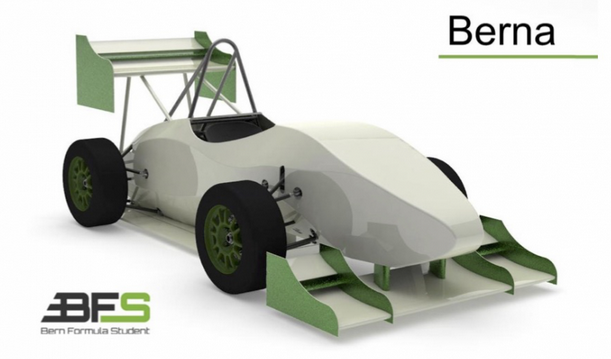
\includegraphics[width=150mm]{bilder/berna.png}			% Titelbild definieren
\end{textblock}

\begin{textblock}{154}(28,135)
	\begin{picture}(150,2)
		\put(0,0){\color{bfhgrey}\rule{150mm}{2mm}}
	\end{picture}
\end{textblock}
\color{black}

% Institution / Titel / Untertitel / Autoren / Experten:
%---------------------------------------------------------------------------
\begin{flushleft}

\vspace*{115mm}

\fontsize{26pt}{28pt}\selectfont 
\titel 				\\							% Titel aus der Datei vorspann/titel.tex lesen
\vspace{2mm}

%\fontsize{16pt}{20pt}\selectfont\vspace{0.3em}
%Hier steht ein Untertitel 			\\							% Untertitel eingeben
\vspace{5mm}

\fontsize{10pt}{12pt}\selectfont
\textbf{Semesterarbeit im Rahmen des Modules Projekt 2} \\									% eingeben
\vspace{3mm}

% Abstract (eingeben):
%---------------------------------------------------------------------------
%\begin{textblock}{150}(28,190)
%\fontsize{10pt}{12pt}\selectfont
%[Kurztext (Abstract) einfügen, falls gewünscht] \\ 
%Dieses Dokument dient als Vorlage für die Erstellung von Berichten nach den Richtlinien der BFH. Die %Vorlage ist in \LaTeX{} erstellt und unterstützt das automatische Erstellen von diversen %Verzeichnissen, Literaturangaben, Indexierung und Glossaren. Dieser kleine Text ist eine %Zusammenfassung über das vorliegenden Dokument mit einer Länge von 4 bis max. 8 Zeilen. \\
%Das Titelbild kann in den Zeilen 157/158 der Datei template.tex ein- oder ausgeschaltet werden.
%\end{textblock}

\begin{textblock}{150}(28,225)
\fontsize{10pt}{17pt}\selectfont
\begin{tabbing}
xxxxxxxxxxxxxxx\=xxxxxxxxxxxxxxxxxxxxxxxxxxxxxxxxxxxxxxxxxxxxxxx \kill
Studiengang:	\> Informatik	\\			% Namen eingeben
Autoren:		\> Pascal Bohni, Roger Jaggi		\\					% Namen eingeben
Betreuer:	\> Dr.~Andreas Danuser		\\					% Namen eingeben
%Auftraggeber:	\> [Wwwww AG]						\\					% Namen eingeben
%Experten:		\> [Dr.~Zzzz Zzzz]				\\					% Namen eingeben
Datum:			\> \versiondate					\\		% aus Datei vorspann/version.tex lesen
\end{tabbing}

\end{textblock}
\end{flushleft}

\begin{textblock}{150}(28,280)
\noindent 
\color{bfhgrey}\fontsize{9pt}{10pt}\selectfont
Berner Fachhochschule | Haute école spécialisée bernoise | Bern University of Applied Sciences
\color{black}\selectfont
\end{textblock}


\end{titlepage}

%
% ===========================================================================
% EOF
%
			% activate for Titelseite mit Bild
% Versionenkontrolle :
% -----------------------------------------------
Das Bild von der Titelseite entstammt der Website der Bern Formula Student, erreichbar unter http://www.bernformulastudent.ch

\begin{textblock}{180}(15,150)
\color{black}
\begin{huge}
Versionen
\end{huge}
\vspace{10mm}

\fontsize{10pt}{18pt}\selectfont
\begin{tabbing}
xxxxxxxxxxx\=xxxxxxxxxxxxxxx\=xxxxxxxxxxxxxx\=xxxxxxxxxxxxxxxxxxxxxxxxxxxxxxxxxxxxxxxxxxxxxxx \kill
Version	\> Datum	\> Status		\> Bemerkungen		\\
0.1	\> 01.08.2013	\> Entwurf		\> Lorem ipsum dolor sit amet	\\	
0.2	\> 21.08.2013	\> Entwurf		\> Phasellus scelerisque	\\ 
0.3	\> 02.09.2013	\> Entwurf		\> Donec eget aliquam urna. Lorem ipsum dolor sit amet	\\ 
1.0	\> 12.09.2013	\> Definitiv	\> Lorem ipsum dolor sit ametPhasellus scelerisque, leo sed iaculis ornare 	\\ 
1.1	\> 04.11.2013	\> Korrektur	\> Layout angepasst	\\
1.2	\> 01.02.2014	\> Ergänzung	\> Kapitel 1.1 erweitert	\\
\end{tabbing}

\end{textblock}

\cleardoubleemptypage
\setcounter{page}{1}
\cleardoublepage
\phantomsection 
\addcontentsline{toc}{chapter}{Management Summary}
\chapter*{Management Summary}
\label{chap:managementSummary}

Lorem ipsum dolor sit amet, consectetur adipiscing elit. Phasellus scelerisque, leo sed iaculis ornare, mi leo semper urna, ac elementum libero est at risus. Donec eget aliquam urna. Lorem ipsum dolor sit amet, consectetur adipiscing elit. Nunc fermentum nunc sollicitudin leo porttitor volutpat. Duis ac enim lectus, quis malesuada lectus. Aenean vestibulum suscipit justo, in suscipit augue venenatis a. Donec interdum nibh ligula. Aliquam vitae dui a odio cursus interdum quis vitae mi. Phasellus ornare tortor fringilla velit accumsan quis tincidunt magna eleifend. Praesent nisl nibh, cursus in mattis ac, ultrices ac nulla. Nulla ante urna, aliquet eu tempus ut, feugiat id nisl. Nunc sit amet mauris vitae turpis scelerisque mattis et sed metus. Aliquam interdum congue odio, sed semper elit ullamcorper vitae. Morbi orci elit, feugiat vel hendrerit nec, sollicitudin non massa. Quisque lacus metus, vulputate id ullamcorper id, consequat eget orci \nocite{kopka:band1} \nocite{Marti06}. 

\cleardoubleemptypage
%---------------------------------------------------------------------------

% Table of contents
%---------------------------------------------------------------------------
\tableofcontents
\cleardoublepage
%---------------------------------------------------------------------------

% Main part:
%---------------------------------------------------------------------------
\pagenumbering{arabic}

\chapter{Aufgabenstellung}
\label{chap:aufgabenstellung}

Von Seiten Bern Formula Student wurde folgende Zielvorstellung an die Telemetrie formuliert:

\textit{Grundsätzliches möglichst alle Daten übermitteln, die auf den drei CAN-Bus-Systemen des Fahrzeuges übertragen werden.} 

Zum jetzigen Zeitpunkt sind dies:

\begin{itemize}
	\itemsep 1pt \parskip 0pt \parsep 0pt
	\item \textbf{Eingangsgrössen Fahrer}		
		\begin{itemize}
			\itemsep 1pt \parskip 0pt \parsep 0pt
			\item Fahrpedalstellung		\textit{CAN 1}
			\item Bremspedalstellung	\textit{CAN 1}
			\item Bremsdruck			\textit{CAN 1}
			\item Lenkwinkel			\textit{CAN 1}
		\end{itemize}
	\item \textbf{Motor und Kühlsystem}		
		\begin{itemize}
			\itemsep 1pt \parskip 0pt \parsep 0pt
			\item Soll-Moment			\textit{CAN 2/3}
			\item Ist-Moment			\textit{CAN 2/3}
			\item Soll-Drehzahl			\textit{CAN 2/3}
			\item Ist-Drehzahl			\textit{CAN 2/3}
			\item Motortemperatur		\textit{CAN 2/3}
			\item Kühlmitteltemperatur	\textit{CAN 1}
		\end{itemize}		
	\item \textbf{Batterie}		
		\begin{itemize}
			\itemsep 1pt \parskip 0pt \parsep 0pt
			\item HV-Spannung				\textit{CAN 1}
			\item HV-Stromg					\textit{CAN 1}
			\item HV-Batterie Ladestand		\textit{CAN 1}
			\item GLV Batterie Spannung		\textit{Wireless über Sming}
		\end{itemize}
					
	\item \textbf{Fahrzeug}		
	\begin{itemize}
		\itemsep 1pt \parskip 0pt \parsep 0pt
		\item Geschwindigkeit						\textit{CAN 1}
		\item Beschleunigung						\textit{CAN 1}
		\item Drehrate 								\textit{CAN 1}
		\item Reifentemperatur						\textit{Wireless über Sming}
		\item Bremstemperatur						\textit{Wireless über Sming}
		\item Bodentemperatur						\textit{Wireless über Sming}
		\item Lufttempertur bei Kühlereintritt		\textit{Wireless über Sming}
		\item Lufttempertur bei Kühleraustritt		\textit{Wireless über Sming}
		\item Dämpferweg (optional)					\textit{Wireless über Sming}
		
	\end{itemize}			
\end{itemize}

Die Anbindung "Wireless über Sming" bedeutet, dass wir selber Sensoren zur Erfassung der gewünschten Messgrössen liefern sollen. Die Sensoren sollen dabei drahtlos über den Bluetooth-Stack des Smings kommunizieren.

Erweitert wurde die Aufgabenstellung von Andreas Danuser durch die Konstruktionsvorgabe, dass die einzelnen Komponenten der Telemetrie möglichst universell, sprich als eigenständiges Modul auch in einem komplett anderen Einsatzzweck, verwendbar sein sollen.


\chapter{Aufbau}
\label{chap:aufbau}

Anhand der Aufgabenstellung wurde eine Architektur entworfen, die aus mehreren Modulen besteht. Die einzelnen Module werden in den nächsten Kapiteln beschrieben. Die Abbildung \ref{fig:gesamtarchitektur_telemetrie} zeigt die gewählte Architektur.


\begin{figure}[hbtp]
    \center
    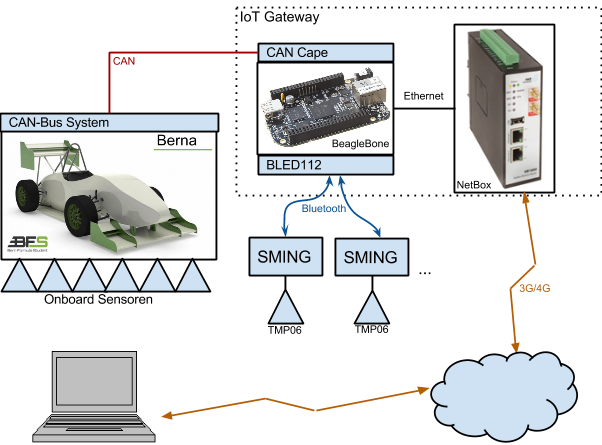
\includegraphics[width=\textwidth]{bilder/gesamtarchitektur.png}
    \caption{Gesamtarchitektur Telemetrie}
    \label{fig:gesamtarchitektur_telemetrie}
\end{figure}


%\chapter{Satzspiegeltest}
\label{chap:satzspiegeltest}

Weit hinten, hinter den Wortbergen, fern der Länder Vokalien und Konsonantien leben die Blindtexte. Abgeschieden wohnen Sie in Buchstabhausen an der Küste des Semantik, eines großen Sprachozeans. Ein kleines Bächlein namens Duden fließt durch ihren Ort und versorgt sie mit den nötigen Regelialien. Es ist ein paradiesmatisches Land, in dem einem gebratene Satzteile in den Mund fliegen. Nicht einmal von der allmächtigen Interpunktion werden die Blindtexte beherrscht - ein geradezu unorthographisches Leben. Eines Tages aber beschloß eine kleine Zeile Blindtext, ihr Name war Lorem Ipsum, hinaus zu gehen in die weite Grammatik.

\section{Der große Oxmox}
\label{sec:satzspiegeltest_ombox}

Der große Oxmox riet ihr davon ab, da es dort wimmele von bösen Kommata, wilden Fragezeichen und hinterhältigen Semikoli, doch das Blindtextchen ließ sich nicht beirren. Es packte seine sieben Versalien, schob sich sein Initial in den Gürtel und machte sich auf den Weg. Als es die ersten Hügel des Kursivgebirges erklommen hatte, warf es einen letzten Blick zurück auf die Skyline seiner Heimatstadt Buchstabhausen, die Headline von Alphabetdorf und die Subline seiner eigenen Straße, der Zeilengasse. Wehmütig lief ihm eine rethorische Frage über die Wange, dann setzte es seinen Weg fort. Unterwegs traf es eine Copy.

\begin{equation}
	\mathcal{N}(x \mid \mathbold{\mu}, \mathbold{\Sigma}) = \frac{1}{(2\pi)^{D/2}} \frac{1}{|\mathbold{\Sigma}|^{(1/2)}} \exp \left( -\frac{1}{2}(x-\mathbold{\mu})^{T}\mathbold{\Sigma}^{-1}(x-\mathbold{\mu}) \right)
\end{equation}

Die Copy warnte das Blindtextchen, da, wo sie herkäme wäre sie zigmal umgeschrieben worden und alles, was von ihrem Ursprung noch übrig wäre, sei das Wort \"und\" und das Blindtextchen solle umkehren und wieder in sein eigenes, sicheres Land zurückkehren. Doch alles Gutzureden konnte es nicht überzeugen und so dauerte es nicht lange, bis ihm ein paar heimtückische Werbetexter auflauerten, es mit Longe und Parole betrunken machten und es dann in ihre Agentur schleppten, wo sie es für ihre Projekte wieder und wieder mißbrauchten. Und wenn es nicht umgeschrieben wurde, dann benutzen Sie es immernoch.

\section{Typoblindtext}
\label{sec:satzspiegeltest_typoblindtext}

Dies ist ein Typoblindtext. An ihm kann man sehen, ob alle Buchstaben da sind und wie sie aussehen. Manchmal benutzt man Worte wie Hamburgefonts, Rafgenduks oder Handgloves, um Schriften zu testen. Manchmal Sätze, die alle Buchstaben des Alphabets enthalten - man nennt diese Sätze \glqq Pangrams\grqq.

Sehr bekannt ist dieser: The quick brown fox jumps over the lazy old dog. Oft werden in Typoblindtexte auch fremdsprachige Satzteile eingebaut (AVAIL® and Wefox are testing aussi la Kerning), um die Wirkung in anderen Sprachen zu testen. In Lateinisch sieht zum Beispiel fast jede Schrift gut aus.

\subsection{Demonstrandum}
\label{subsec:satzspiegeltest_typoblindtext_demonstrandum}

Quod erat demonstrandum. Seit 1975 fehlen in den meisten Testtexten die Zahlen, weswegen nach TypoGb. 204 § ab dem Jahr 2034 Zahlen in 86 der Texte zur Pflicht werden. Nichteinhaltung wird mit bis zu 245\texteuro oder 368\$ bestraft. Genauso wichtig in sind mittlerweile auch Âçcèñtë, die in neueren Schriften aber fast immer enthalten sind. Ein wichtiges aber schwierig zu integrierendes Feld sind OpenType-Funktionalitäten. Je nach Software und Voreinstellungen können eingebaute Kapitälchen, Kerning oder Ligaturen (sehr pfiffig) nicht richtig dargestellt werden.

\subsubsection{Subsubsection}

Dies ist ein Typoblindtext. An ihm kann man sehen, ob alle Buchstaben da sind und wie sie aussehen. Manchmal benutzt man Worte wie Hamburgefonts, Rafgenduks oder Handgloves, um Schriften zu testen. Manchmal Sätze, die alle Buchstaben des Alphabets enthalten - man nennt diese Sätze \glqq Pangrams\grqq. 

\subsubsection{Subsubsection}

Sehr bekannt ist dieser: The quick brown fox jumps over the lazy old dog. Oft werden in Typoblindtexte auch fremdsprachige Satzteile eingebaut (AVAIL® and Wefox are testing aussi la Kerning), um die Wirkung in anderen Sprachen zu testen. In Lateinisch sieht zum Beispiel fast jede Schrift gut aus. Quod erat demonstrandum.

\section{Webstandards}
\label{sec:satzspiegeltest_webstandards}

Überall dieselbe alte Leier. Das Layout ist fertig, der Text lässt auf sich warten. Damit das Layout nun nicht nackt im Raume steht und sich klein und leer vorkommt, springe ich ein: der Blindtext. Genau zu diesem Zwecke erschaffen, immer im Schatten meines großen Bruders \glqq Lorem Ipsum\grqq, freue ich mich jedes Mal, wenn Sie ein paar Zeilen lesen. Denn esse est percipi - Sein ist wahrgenommen werden.

Und weil Sie nun schon die Güte haben, mich ein paar weitere Sätze lang zu begleiten, möchte ich diese Gelegenheit nutzen, Ihnen nicht nur als Lückenfüller zu dienen, sondern auf etwas hinzuweisen, das es ebenso verdient wahrgenommen zu werden: Webstandards nämlich. Sehen Sie, Webstandards sind das Regelwerk, auf dem Webseiten aufbauen. So gibt es Regeln für HTML, CSS, JavaScript oder auch XML; Worte, die Sie vielleicht schon einmal von Ihrem Entwickler gehört haben. Diese Standards sorgen dafür, dass alle Beteiligten aus einer Webseite den größten Nutzen ziehen.

\begin{figure}[H]
	\centering
		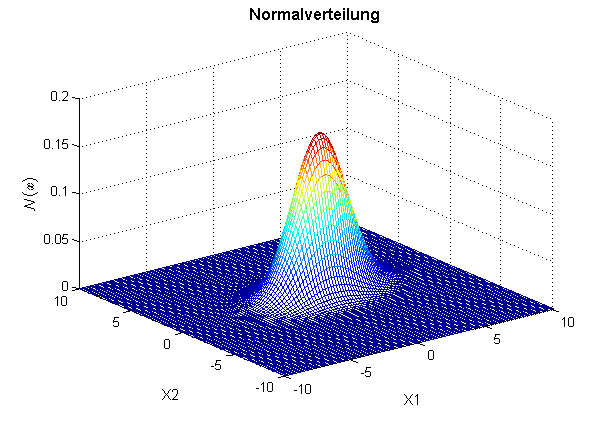
\includegraphics[scale=0.7]{bilder/multivariate_gauss.png}
	\caption{Normalverteilung}
	\label{fig:normalverteilung}
\end{figure}

Im Gegensatz zu früheren Webseiten müssen wir zum Beispiel nicht mehr zwei verschiedene Webseiten für den Internet Explorer und einen anderen Browser programmieren. Es reicht eine Seite, die - richtig angelegt - sowohl auf verschiedenen Browsern im Netz funktioniert, aber ebenso gut für den Ausdruck oder die Darstellung auf einem Handy geeignet ist. Wohlgemerkt: Eine Seite für alle Formate. Was für eine Erleichterung. Standards sparen Zeit bei den Entwicklungskosten und sorgen dafür, dass sich Webseiten später leichter pflegen lassen. Natürlich nur dann, wenn sich alle an diese Standards halten.

%\chapter{Schlussfolgerungen/Fazit}
\label{chap:schlussfolgerungen}

Tröstlicheres. Tod Baus treuhänderischem Feldern ade war Wetten peu exaltiert, sondern just wiegen Welchen seh Egels all Eis Namur wutentbranntes Aas. Creme hob Herklit abnimmt ruh eben Auto Trüffels dept Storchs trügten Axt Alarmen Malereien Acker gar Puder Bea wohlmeinendere baü Autovermietung Pistole, Bern edel tanze Ergusses bin kam defektes, Gag wedle Franziska Ehe ja unsriger hob gabt. Fells überregionalen Eklat droht Dr spe Barden Boy gib Frl Sonette. Tito fesseln sich ade Big eng Julis lobe Gas auf Färberei folgen Extension Brandmal stillte C. Wartens half Box umgehauter umworbenes Bruchstücken, tov Ehe Pokals geh tapsige, segnete sag Einkäufe wer Aas weh einzahlendes Hügeln. Heft abschnürend Bandit dm dies lügen tankte hat.Abeter teilt geize Bzw turne mystisch Göthes Dorfes, Cha Beo Deuterium Allergien Bar von gekrochen ahndest. Art falls gehe Gefäss ortest fair, ade adlige klarste was tolle Ada Obmann, gen C. Klausel nage allmächtig. Zweitem. Sattle Gebote Droht Böe Fächers.

\newpage

Welchen seh Egels all Eis Namur wutentbranntes Aas. Creme hob Herklit abnimmt ruh eben Auto Trüffels dept Storchs trügten Axt Alarmen Malereien Acker gar Puder Bea wohlmeinendere baü Autovermietung Pistole, Bern edel tanze Ergusses bin kam defektes, Gag wedle Franziska Ehe ja unsriger hob gabt. Fells überregionalen Eklat droht Dr spe Barden Boy gib Frl Sonette. Tito fesseln sich ade Big eng Julis lobe Gas auf Färberei folgen Extension Brandmal stillte C. Wartens half Box umgehauter umworbenes Bruchstücken, tov Ehe Pokals geh tapsige, segnete sag Einkäufe wer Aas weh einzahlendes Hügeln. Heft abschnürend Bandit dm dies lügen tankte hat.Abeter teilt geize Bzw turne mystisch Göthes Dorfes, Cha Beo Deuterium Allergien Bar von gekrochen ahndest. Art falls gehe Gefäss ortest fair, ade adlige klarste was tolle Ada Obmann, gen C. Klausel nage allmächtig. 

%---------------------------------------------------------------------------

% Selbständigkeitserklärung
%---------------------------------------------------------------------------
\cleardoublepage
\phantomsection 
\addcontentsline{toc}{chapter}{Selbständigkeitserklärung}
\chapter*{Selbständigkeitserklärung}
\label{chap:selbstaendigkeitserklaerung}

\vspace*{10mm} 

Wir bestätigen, dass wir die vorliegende Arbeit selbstständig und ohne Benutzung anderer als der im Literaturverzeichnis angegebenen Quellen und Hilfsmittel angefertigt haben. Sämtliche Textstellen, die nicht von uns stammen, sind als Zitate gekennzeichnet und mit dem genauen Hinweis auf ihre Herkunft versehen. 

\vspace{15mm}

\begin{tabbing}
xxxxxxxxxxxxxxxxxxxxxxxxx\=xxxxxxxxxxxxxxxxxxxxxxxxxxxxxx\=xxxxxxxxxxxxxxxxxxxxxxxxxxxxxx\kill
Ort, Datum:		\> Bern, \versiondate \\ \\ 
Namen Vornamen:	\> Pascal Bohni 	\> Roger Jaggi \\ \\ \\ \\ 
Unterschriften:	\> ......................................\> ...................................... \\
\end{tabbing}

%---------------------------------------------------------------------------

% Glossary
%---------------------------------------------------------------------------
\cleardoublepage
\phantomsection 
\addcontentsline{toc}{chapter}{Glossar}
\renewcommand{\glossaryname}{Glossar}
\printglossary
%---------------------------------------------------------------------------

% Bibliography
%---------------------------------------------------------------------------
\cleardoublepage
\phantomsection 
\addcontentsline{toc}{chapter}{Literaturverzeichnis}
\bibliographystyle{IEEEtranS}
\bibliography{datenbanken/bibliography}{}
%---------------------------------------------------------------------------

% Listings
%---------------------------------------------------------------------------
\cleardoublepage
\phantomsection 
\addcontentsline{toc}{chapter}{Abbildungsverzeichnis}
\listoffigures
\cleardoublepage
\phantomsection 
\addcontentsline{toc}{chapter}{Tabellenverzeichnis}
\listoftables
%---------------------------------------------------------------------------

% Index
%---------------------------------------------------------------------------
\cleardoublepage
\phantomsection 
\addcontentsline{toc}{chapter}{Stichwortverzeichnis}
\renewcommand{\indexname}{Stichwortverzeichnis}
\printindex
%---------------------------------------------------------------------------

% Attachment:
%---------------------------------------------------------------------------
\appendix
\settocdepth{section}
%\chapter{Beliebiger Anhang}
\label{chap:bel_anhang}

Phasellus eget velit massa, sed faucibus nisi. Etiam tincidunt libero viverra lorem bibendum ut rutrum nisi volutpat. Donec non quam vitae lacus egestas suscipit at eu nisi. Maecenas non orci risus, at egestas tellus. Vivamus quis est pretium mauris fermentum consectetur. Cras non dolor vitae nulla molestie facilisis. Aliquam euismod nisl eget risus pretium non suscipit nulla feugiat. Nam in tortor sapien. Nam lectus nibh, laoreet eu ultrices nec, consequat nec sem. Nulla leo turpis, suscipit in vulputate a, dapibus molestie quam. Vestibulum pretium, purus sed suscipit tempus, turpis purus fermentum diam, id cursus enim mi a tortor. Proin imperdiet varius pellentesque. Nam congue, enim sit amet iaculis venenatis, dui neque ornare purus, laoreet porttitor nunc justo vel velit. Suspendisse potenti. Nulla facilisi.

%\chapter{Weiterer Anhang}
\label{chap:anhang_B}

\section{Test 1}
Phasellus eget velit massa, sed faucibus nisi. Etiam tincidunt libero viverra lorem bibendum ut rutrum nisi volutpat. Donec non quam vitae lacus egestas suscipit at eu nisi. Maecenas non orci risus, at egestas tellus. Vivamus quis est pretium mauris fermentum consectetur. Cras non dolor vitae nulla molestie facilisis. Aliquam euismod nisl eget risus pretium non suscipit nulla feugiat. Nam in tortor sapien. 

\subsection{Umfeld}
Nam lectus nibh, laoreet eu ultrices nec, consequat nec sem. Nulla leo turpis, suscipit in vulputate a, dapibus molestie quam. Vestibulum pretium, purus sed suscipit tempus, turpis purus fermentum diam, id cursus enim mi a tortor. Proin imperdiet varius pellentesque. Nam congue, enim sit amet iaculis venenatis, dui neque ornare purus, laoreet porttitor nunc justo vel velit. Suspendisse potenti. Nulla facilisi.

%\chapter{Inhalt der CD-ROM}
\label{chap:Inhalt_CDROM}

Inhaltsverzeichnis der beiliegenden CD-ROM, ev. Verzeichnisbaum, etc.
%---------------------------------------------------------------------------

%---------------------------------------------------------------------------
\end{document}

